\chapter{Introduction au Schémas Compactes}
\section{Cas d'une dimension d'espace}
\subsection*{\underline{Domaine et Discrétisation}:}
On considère un intervalle périodique \(\Omega = [0,L]\), qu'on discrétise en \(N\) points également espacés, notés \(x_i\) pour \(i = 0, 1, \ldots, N-1\).
\[0=x_0<x_1<\ldots<x_{N-1}< L, \hspace{7mm} \text{avec } \hspace{5mm} x_i=ih, \hspace{5mm} h=\frac{L}{N} \]
\[\hspace{5mm} x_{N}=x_0 \hspace{5mm} \text{(mod L.)}\]

\vspace{0.4cm}
\begin{figure}[h!]
    \centering
        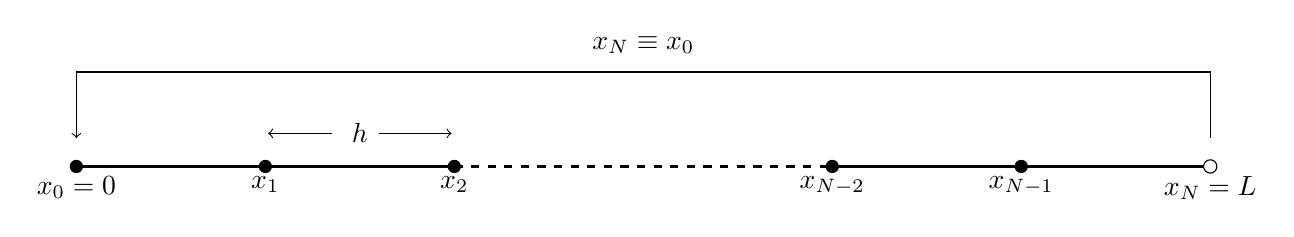
\begin{tikzpicture}[scale=1.2]
    % Draw the axis
   \draw[-,thick] (0,0) -- (4,0);
    \draw[dashed, thick] (4,0) -- (8,0);
    \draw[-,thick] (8,0) -- (12,0);
    

    % Grid points
    \draw[->, shorten >=1pt] (2.7,0.35) -- (2,0.35);
    \draw[->, shorten >=1pt] (3.2,0.35) -- (4,0.35);
    \node[] at (3,0.35) {$h$};
    \foreach \x in {0,2,4,8,10,12}{
        \fill (\x,0) circle (2pt);
    }
    \filldraw[fill=white, draw=black] (12,0) circle (2pt) node[below] {$x_N=L$};

    % Labels
    \node[below] at (0,0) {$x_0=0$};
    \node[below] at (2,0) {$x_1$};
    \node[below] at (4,0) {$x_2$};
    \node[below] at (8,0) {$x_{N-2}$};
    \node[below] at (10,0) {$x_{N-1}$};

    \draw[->]
    (12,0.3) -- (12,1) --(0,1) node[midway,above=3pt] {$x_N \equiv x_0$} -- (0,0.3);

    \end{tikzpicture}
    \caption{\textit{Discrétisation de l’intervalle périodique \(\Omega = [0,L]\) en \(N\) points.}}
\label{fig:periodic_discretization}
\end{figure}

\subsubsection*{\underline{Schémas Compactes}:}

